\section{System Architecture Design}
There have been previous systems like ESA's MARS-M module that have powder transportation functionality but there is little detail on how they did it available to the public. Therefore, the many well documented terrestrial methods and the required adaptations to microgravity were reviewed and compared.

Five common methods of powder dispensing were identified: Screw Fed, Vibration Fed, Liquid Suspension Fed, Rotating Disk Fed and Positive Displacement Fluidized Powder Bed. Basic diagrams of the different methods are shown in \autoref{fig:powder-dispensing-methods}. 
\begin{figure}[htbp]
    \centering

    % First row: 3 images
    \begin{minipage}{0.3\textwidth}
        \centering
        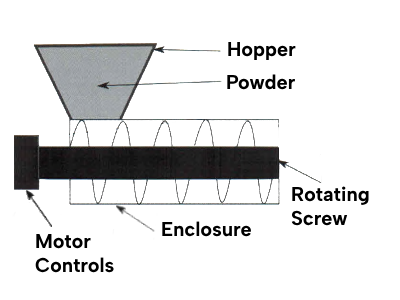
\includegraphics[width=\textwidth]{../report_assets/screw_feed_polished.png}
        \caption*{(a) Screw Fed Design}
    \end{minipage}
    \hfill
    \begin{minipage}{0.3\textwidth}
        \centering
        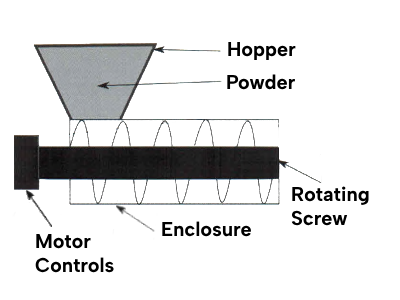
\includegraphics[width=\textwidth]{../report_assets/screw_feed_polished.png}
        \caption*{(b) Vibration Fed Design}
    \end{minipage}
    \hfill
    \begin{minipage}{0.3\textwidth}
        \centering
        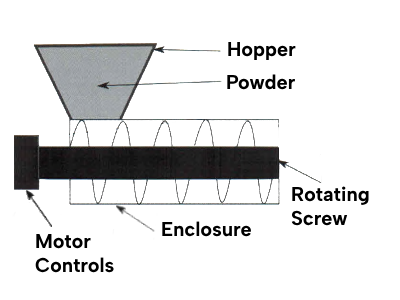
\includegraphics[width=\textwidth]{../report_assets/screw_feed_polished.png}
        \caption*{(c) Liquid Suspension Design}
    \end{minipage}

    \vspace{0.5cm} % space between top and bottom rows

    % Second row: 2 images
    \begin{minipage}{0.4\textwidth}
        \centering
        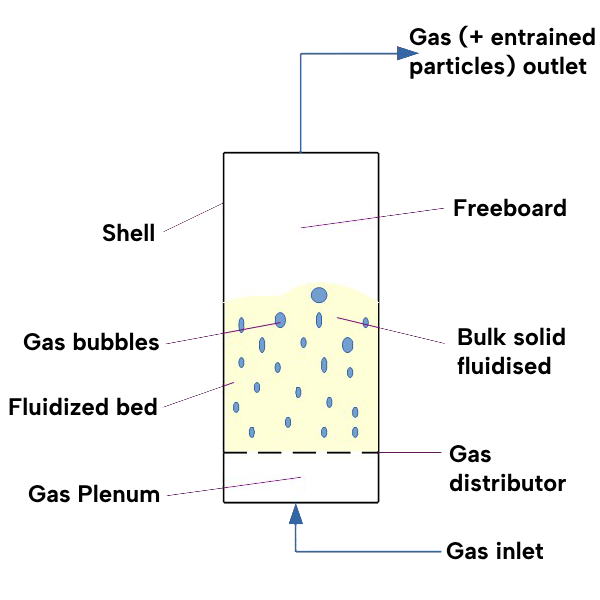
\includegraphics[width=\textwidth]{../report_assets/Fluidized_Bed_polished.png}
        \caption*{(d) Rotating Disk Design}
    \end{minipage}
    \hspace{0.1\textwidth}
    \begin{minipage}{0.4\textwidth}
        \centering
        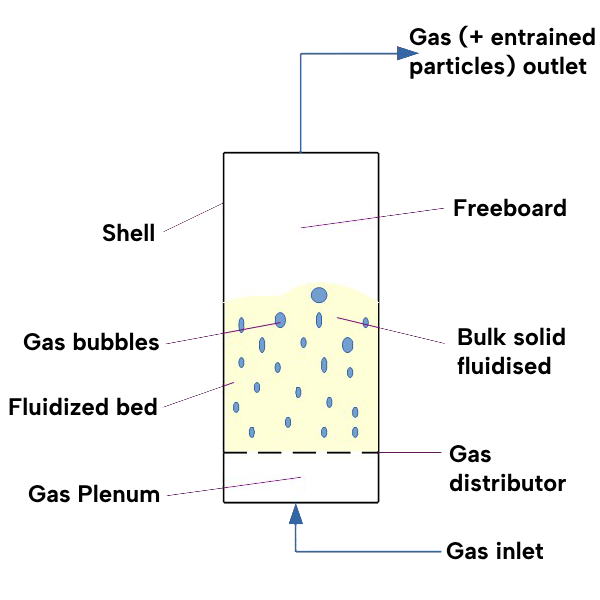
\includegraphics[width=\textwidth]{../report_assets/Fluidized_Bed_polished.png}
        \caption*{(e) Fluidized Powder Bed Design}
    \end{minipage}

    \caption{Overall figure caption describing all subfigures.}
    \label{fig:powder-dispensing-methods}
\end{figure}

The most promising methods were Screw Fed and Fluidized Powder Bed. The whole tabulated comparison of the methods can be seen in \autoref{appendix:feed-architecture-analysis}.
% After selecting the architecture of Fluidized Powder Bed, a deeper dive into the usage and physics was conducted. 



\section{Gas Permeable Pistons}
Fluidising powder feed systems were typically designed to fluidise a local region near the outlet of the tank and then a seperate piston was electrically actuated to force powder out at a controlled rate. A benefit of this method is that it is simple to implement but it incurs mass penalties of the heavy motor and requires additional considerations of power and motor control. An improvement upon this implementation is leveraging the fact that pressure lines are already present in the design, therefore the piston can be controlled pneumatically through the pressure differential across the piston head. Even further still, the carrier gas and piston pressurant gas can be combined if the piston head is permeable. This simplifies the design again.

\begin{figure}[htbp]
    \centering

    \begin{minipage}{0.45\textwidth}
        \centering
        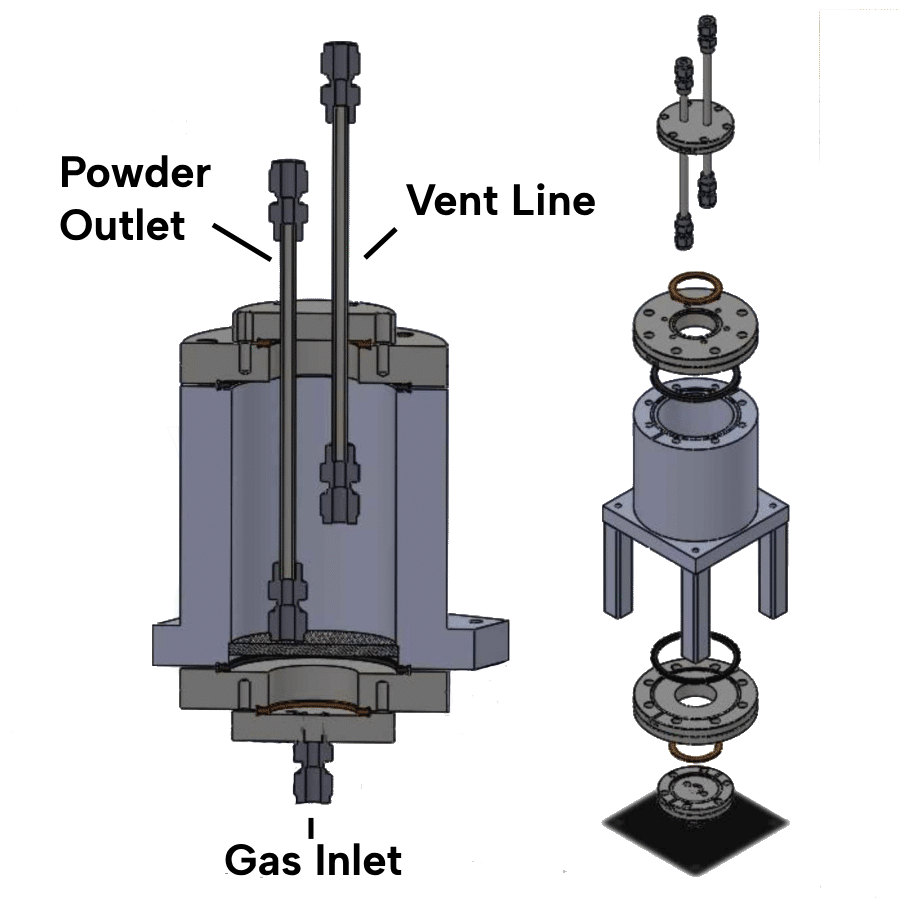
\includegraphics[width=\textwidth]{../report_assets/COSMOS_DIAGRAM.png}
        \caption{FSI of piston head.}
        \label{fig:fluent-fsi-piston-head}
    \end{minipage}
    \hfill
    \begin{minipage}{0.45\textwidth}
        \centering
        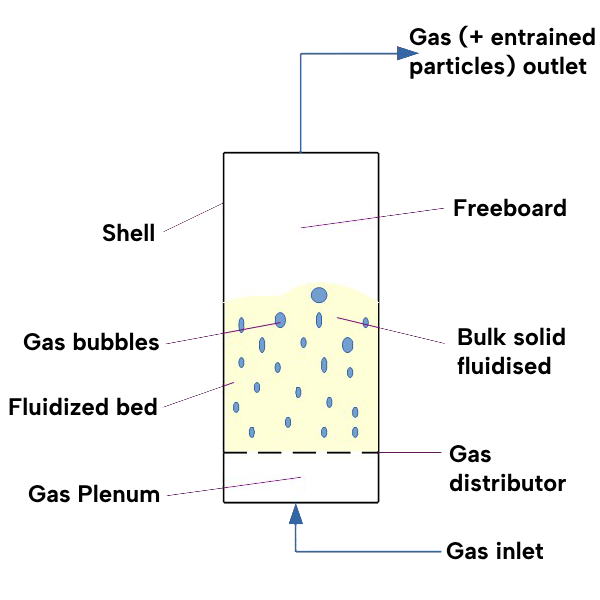
\includegraphics[width=\textwidth]{../report_assets/Fluidized_Bed_polished.png}
        \caption{FSI of piston head + powder.}
        \label{fig:fluent-fsi-piston-head-powder}
    \end{minipage}

\end{figure}

Geometry for piston, cocking issue
NEED TO FIND PAPER CORRELATING MASS FLOW TO PISTON force
\newpage
\section{System Physics}
One could expect to model a system like this by combining previous data and insight of how the motor actuated fluidised system works and then augmenting this due to the pneumatic actuation of the piston. However, previous investigations into this [cite] seem to suggest that there is no such correlation between force applied to the piston and mass flow rate of the powder. 

\begin{figure}[htbp]
    \centering

    \begin{minipage}{0.3\textwidth}
        \centering
        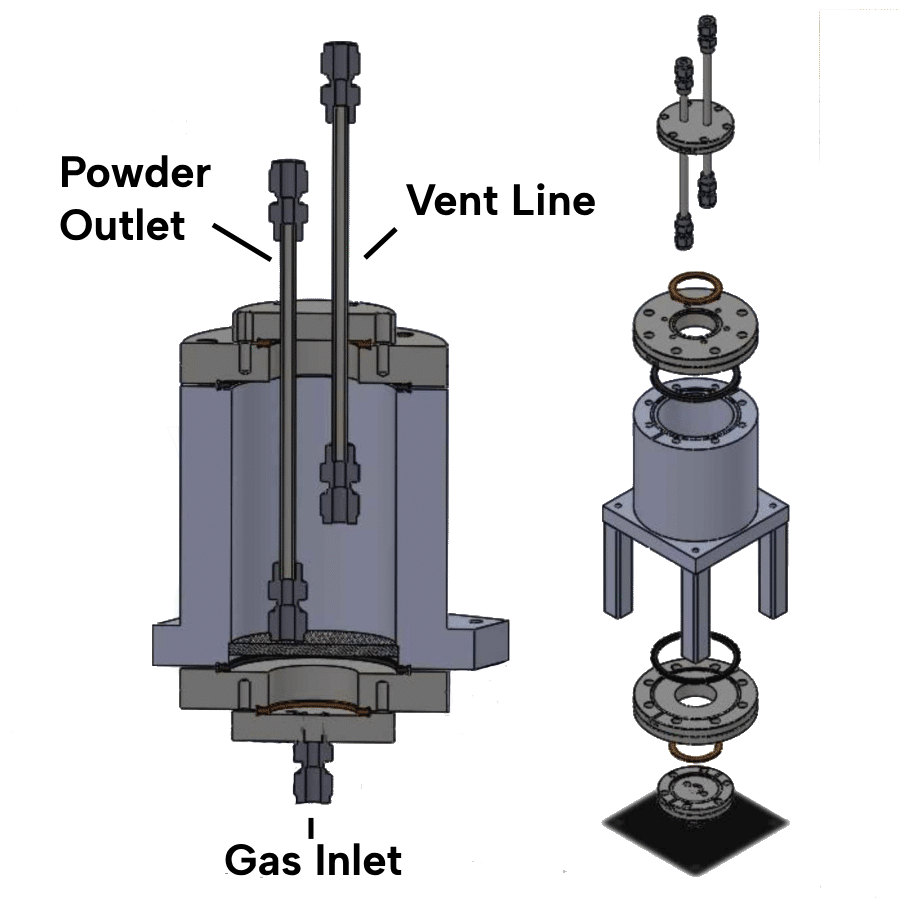
\includegraphics[width=\textwidth]{../report_assets/COSMOS_DIAGRAM.png}
        \caption{Current feed system diagram.}\label{fig:current-feed-system-exploded-diagram}
    \end{minipage}
    \hfill
    \begin{minipage}{0.3\textwidth}
        \centering
        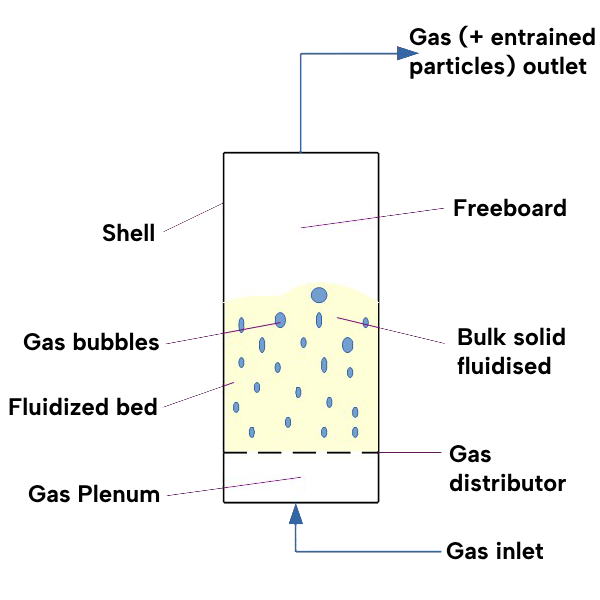
\includegraphics[width=\textwidth]{../report_assets/Fluidized_Bed_polished.png}
        \caption{Simplified fluidized powder bed diagram.}\label{fig:fluidized-bed-diagram}
    \end{minipage}
    \hfill
    \begin{minipage}{0.3\textwidth}
        \centering
        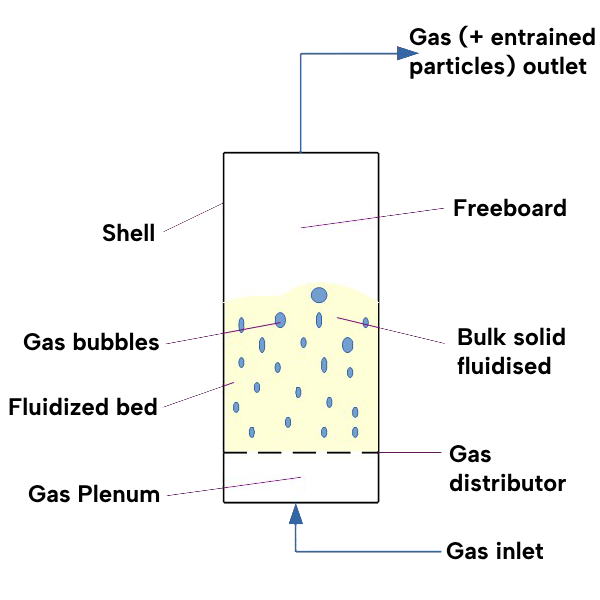
\includegraphics[width=\textwidth]{../report_assets/Fluidized_Bed_polished.png}
        \caption{Current design with turbulent inlet.}\label{fig:current-feed-system-fluent}
    \end{minipage}

\end{figure}
It is expected that this is because the PT is too far downstream and the powder inbetween is lowering the pressure. Using data given for the experimentation and the pressure drop expected from the cylindrical powder section alone
it has previously been reported that there is not a simple linear relationship between the force of the piston on the powder and the 

% lowkey weak argument look for better

Another argument about piston force VS mass flow rate

alternatively there is a strong linear correlation between velocity of piston head and mass flow rate of powder. This is well defined and could be used instead of the force


The physics is hopefully understood as a non-linear combination of the two effects. Gas applying a force to the piston and the fluidisation of the powder. If we look at the system as though it is not gas permiable then we would expect it to look like this. Given the piston head is though, we expect it to change in this way.

At the end of the day, this system is similar to other systems investiaged. It varies in 1 key way, the fact that since it is going into a nozzle then a vacuum in the LPCS process there is no combustion chamber to provide backpressure.
\section{Experimental Setup}
Low pressures were investiaged.
\begin{figure}[htbp]
    \centering

    \begin{minipage}{0.45\textwidth}
        \centering
        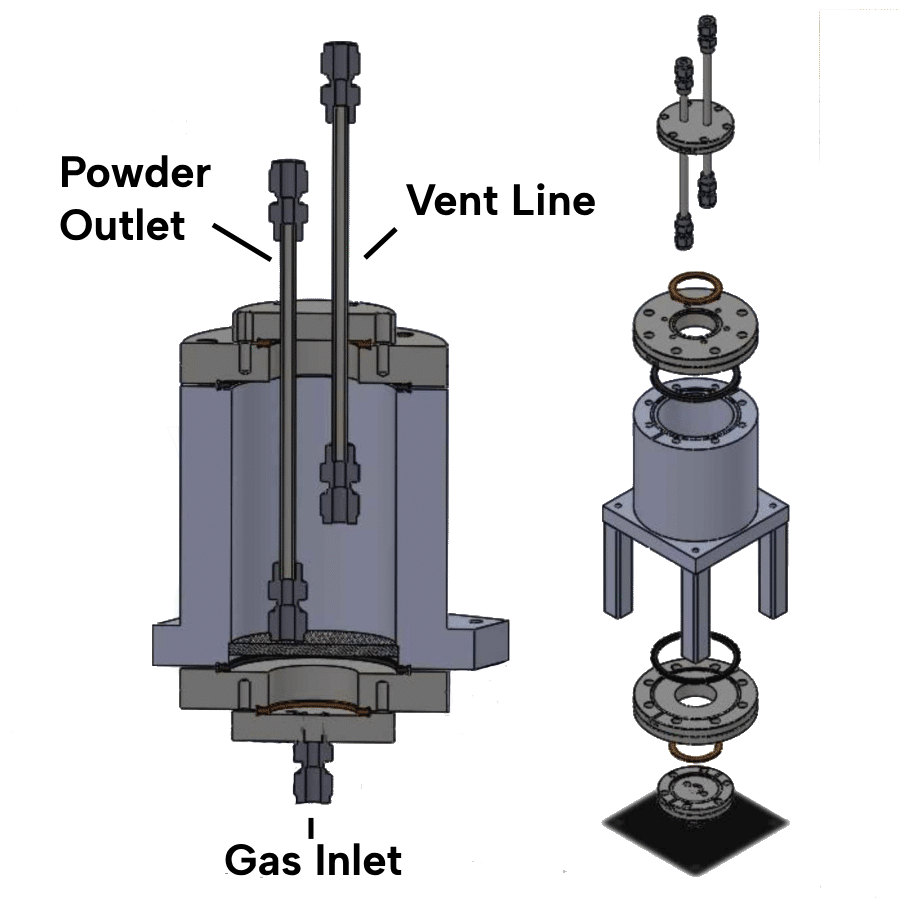
\includegraphics[width=\textwidth]{../report_assets/COSMOS_DIAGRAM.png}
        \caption{Systems diagram.}
        \label{fig:systems-diagram}
    \end{minipage}
    \hfill
    \begin{minipage}{0.45\textwidth}
        \centering
        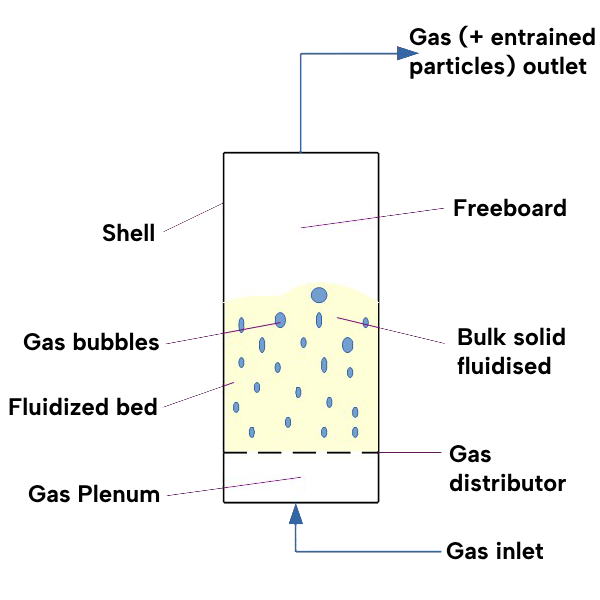
\includegraphics[width=\textwidth]{../report_assets/Fluidized_Bed_polished.png}
        \caption{Pic of experiment.}
        \label{fig:experiment-image}
    \end{minipage}

\end{figure}

\newpage
\section{Hopper tank design}

\section{Choke Point}
It is proposed that the flow characteristics of the fluidised powder bed system are simpler, therefore easier to control, if the flow is choked. This chokepoint then needs to withstand getting sand blasted as to not change the throat area over time. The most ideal solution to this problem involves very hard materials like ... or ... that can withstand the powder for many tests. Given the scope of this project, however, one-time use 3D printed chokepoints were used. They were made of PLA which has a hardness of ... and is expected to wear away at a rate of .... This was deemed experimentally acceptable because of a change in throat diameter of ... over ... doesnt significantly alter the results.

\newpage
\section{Cyclone seperator and measurement method}
Typical literature ways of measuring powder mass flow rate is through Displacement of the piston. This paper [cite] shows that other methods equally as effective are measuring the mass of powder leaving. This project does the latter through the use of a cyclone seperator.

Cyclone seperators work like this

measurement of the mass changes was done through 3 load cells shown in figure blah

If needed could take vid of experiment and look at piston displacement but probs not

\section{Data acuisition and actuators}
Data aquisition was done through ICLR SRAD boards. The sensors were calibrated soon before the experiment but through no rigorous method. Area for improvement.

The data was then sent to a grafana dashboard and this also allowed for actuation of the solenoid valve for clean operations.

\newpage
\section{Testing operations}

\section{Powder}
For safety and due to the limited budget, sand was used as the powder. This is one of the greatest areas for improvement, i dont actually know what size the powder is or the distribution of those sizes. This powder has been measured to have [density = 1.4g/cm3]